%% Measurement-validity study of bias injection/removal asymmetry.
%% Target: The European Journal on Artificial Intelligence (SAGE).
%% Compiles with pdflatex; references via SageH.bst (Harvard author-year).
\documentclass[Afour,sageh,times]{sagej}

\usepackage{booktabs}
\usepackage{adjustbox}
\usepackage{graphicx}
\usepackage{multirow}
\usepackage{amsmath}
\usepackage{amssymb}
\usepackage{url}

\setcounter{secnumdepth}{3}

\begin{document}

\runninghead{Deb}

\title{Step-count ratios do not measure bias hysteresis: a matched-objective control for multilingual encoder models}

\author{Koushik Deb\affilnum{1}}

\affiliation{\affilnum{1}Indian Institute of Information Technology Kalyani, West Bengal, India}

\corrauth{Koushik Deb, Indian Institute of Information Technology Kalyani, Kalyani, West Bengal, 741235, India.}

\email{koushik\_phd21@iiitkalyani.ac.in}

\begin{abstract}
Debiasing pipelines for language models often assume that removing a social bias costs about as much as introducing it. Recent studies question that assumption and report an asymmetry: bias removal appears to need more gradient steps than bias injection, a pattern described as bias hysteresis. The measure of this asymmetry, the ratio $R = T_{\mathrm{debias}} / T_{\mathrm{bias}}$, is computed from step counts that can be right-censored when a threshold is never crossed, and the forward and reverse paths often optimise two different loss functions. This work tests the asymmetry on the same grid under two objectives: a mismatched objective that reproduces the original protocol, and a matched objective in which injection and removal drive the same signed log-probability gap in opposite directions. Experiments cover five multilingual encoder models, three languages (English, Hindi, and Bengali), four bias categories, and three seeds, giving 180 conditions per objective. Neither objective shows the asymmetry once censoring is handled and the median replaces the mean. Under the matched objective the median $R$ is 0.393, with a model-clustered 95\% confidence interval of [0.359, 0.426]; under the mismatched objective it is 0.074. Both reject symmetry in the direction $R < 1$ (Wilcoxon on $\log R$, $p < 10^{-14}$): removal is faster than injection, not slower. The reported $R > 1$ traces to two measurement choices. The mismatched objective fails to cross the threshold in 27\% of conditions, and these censored cases enter the original average at the ceiling value; the mean then sits above one while the median stays below. Step-count ratios do not measure bias hysteresis, and an asymmetry claim needs censoring-aware, median-based analysis under a matched objective before it can stand.
\end{abstract}

\keywords{Language model bias, multilingual fairness, bias mitigation, measurement validity, responsible AI}

\maketitle

\section{Introduction}
\label{sec:introduction}

Social biases in language models raise concern as these models enter hiring tools, content moderation, and education \citep{blodgett2020language}. Stereotypical associations learned during pretraining carry into downstream use and can amplify existing inequalities \citep{caliskan2017semantics}. A large body of work detects such biases and proposes methods to remove them \citep{bolukbasi2016man, ravfogel2020null, schick2021selfdiagnosis}.

Most of this work assumes that the effort to remove a bias is comparable to the effort to introduce it. A model pushed towards a stereotype over a fixed number of gradient steps is expected to recover over a similar number of steps. Recent studies question that assumption. They inject a bias and then remove it, to study acquisition and unlearning as distinct processes \citep{islam2025biasgym, liu2025rethinking}. A natural summary of such an inject-then-remove protocol is the step-count ratio $R = T_{\mathrm{debias}} / T_{\mathrm{bias}}$, where $T_{\mathrm{bias}}$ is the step count to push a bias score above a threshold and $T_{\mathrm{debias}}$ is the step count to bring it back below. When removal takes more steps than injection, so that $R > 1$, the protocol is read as showing an asymmetry between acquisition and unlearning. By analogy with physical systems whose state depends on history, this asymmetry is called bias hysteresis.

The ratio carries two measurement problems that its interpretation overlooks. The first is censoring. When injection does not reach the threshold within its step budget, $T_{\mathrm{bias}}$ is capped; when removal does not return below the threshold, $T_{\mathrm{debias}}$ is capped. A capped ratio is a right-censored lower bound, not a measurement, yet a mean taken over such values treats the cap as a real number and pulls the average up. The second is the objective. Injection and removal are often optimised with different loss functions, one using masked-language-model cross-entropy on stereotypical targets and the other a squared difference between stereotypical and anti-stereotypical log-probabilities. These losses differ in gradient scale, so a step under one is not comparable to a step under the other.

This study tests the asymmetry on one grid under two objectives. The mismatched objective reproduces the original protocol, with cross-entropy injection and squared-gap removal. The matched objective optimises the same signed log-probability gap in both directions, so the two paths differ only in sign. Every other setting is held fixed: the same optimiser, learning rate, low-rank adapter configuration, and evaluation schedule. Crossing times are estimated by interpolation and censored cases are excluded rather than capped, and the median replaces the mean. We evaluate both objectives across five multilingual encoder models, three languages, four bias categories, and three seeds, and record gradient norms so that any residual asymmetry stays visible.

This paper makes two contributions. It introduces a matched-objective, censoring-aware protocol for injection--removal asymmetry and applies it on the same 180-condition grid as the original mismatched protocol, across five multilingual encoders and three languages. It shows that the reported $R > 1$ does not survive proper analysis under either objective: the median $R$ is 0.393 under the matched objective and 0.074 under the mismatched one, and the earlier $R > 1$ traces to censored conditions entering a mean at the ceiling value rather than to any property of the model.

\section{Related work}
\label{sec:related}

Bias in language models has been studied since word-embedding work showed that distributional semantics absorb human stereotypes \citep{caliskan2017semantics, bolukbasi2016man}. The concern carries into contextual models. Benchmarks such as StereoSet \citep{nadeem2021stereoset}, CrowS-Pairs \citep{nangia2020crowspairs}, and Indian-BhED \citep{khandelwal2023indianbhed} measure stereotypical preference across categories and languages. \citet{kaneko2022unmasking} proposed the Average Unmasked Likelihood to avoid frequency effects in masked-language-model scoring. \citet{blodgett2021stereotyping} showed that several pair-based benchmarks contain confounds, which cautions against reading any single derived number as a clean signal.

Debiasing methods span several mechanism classes. Counterfactual Data Augmentation retrains on swapped demographic terms \citep{zmigrod2019counterfactual}. Iterative Nullspace Projection removes bias directions from representations \citep{ravfogel2020null}. Self-Debias adjusts decoding without weight updates \citep{schick2021selfdiagnosis}. Weight-editing methods such as DAMA \citep{limisiewicz2024dama} and BiasEdit \citep{xu2025biasedit} modify targeted parameters directly. \citet{meade2022empirical} compared these methods and found that measured effectiveness depends heavily on the evaluation setup, which again points to measurement sensitivity.

The claim that removal costs more than injection appears in two recent lines of work. \citet{islam2025biasgym} inject and then remove bias with component-level identification. \citet{liu2025rethinking} study asymmetric removal cost in machine unlearning. Neither controls for the objective used in each direction, so neither separates a genuine asymmetry from a difference between two loss functions. Work on intrinsic and extrinsic bias metrics reports a related gap. \citet{goldfarbtarrant2021intrinsic} found that intrinsic bias scores do not predict downstream bias, and \citet{delobelle2022measuring} found that fairness measurements shift with the probing choice. This study extends that scrutiny from static scores to a dynamic quantity, the step-count ratio, and asks whether it measures what its name claims.

\section{Method}
\label{sec:methodology}

Measuring an asymmetry between two training directions requires that the two directions be comparable. We first define the bias score and the ratio, then describe the matched objective that makes the comparison fair.

\subsection{Models, data, and bias score}

The study evaluates five multilingual encoder models: mBERT \citep{devlin2019bert}, XLM-RoBERTa \citep{conneau2020unsupervised}, MuRIL \citep{khanuja2021muril}, IndicBERTv2, and mmBERT. All five support English, Hindi, and Bengali. Each model is fine-tuned with low-rank adapters \citep{hu2022lora} of rank 16, so that injection and removal modify the same small parameter set and start from the same pretrained weights.

Bias is drawn from two benchmarks. Multi-CrowS-Pairs \citep{nangia2020crowspairs} provides sentence pairs across Western-framed categories, and an Indian-context set derived from Indian-BhED \citep{khandelwal2023indianbhed} adds caste, gender, religion, and race. Both are extended to Hindi and Bengali through translation with back-translation checks. We report on four categories with adequate sample counts: race-colour, religion, nationality, and socioeconomic status. Each item is a masked sentence with a stereotypical and an anti-stereotypical target, for example \textit{All the dirty and petty jobs are done by} \texttt{[MASK]}, with targets \textit{Dalits} and \textit{Brahmins}. Parallel Hindi and Bengali items exist for every English item in the caste, gender, religion, and race categories.

The bias score uses the Average Unmasked Likelihood \citep{kaneko2022unmasking}. For a sentence pair, the score compares the pseudo-log-likelihood of the stereotypical and anti-stereotypical completions at the masked position, mapped to $[0,1]$; a value above 0.5 marks stereotypical preference. We denote this score $B$.

\subsection{The asymmetry ratio}

Bias injection trains the model until its bias score first exceeds a threshold $\theta$. The step count at that crossing is $T_{\mathrm{bias}}$. Bias removal then trains from the injected checkpoint until the score falls back below $\theta$, giving $T_{\mathrm{debias}}$. The asymmetry ratio is
\begin{equation}
R = \frac{T_{\mathrm{debias}}}{T_{\mathrm{bias}}},
\label{eq:R}
\end{equation}
where $R > 1$ means removal takes more steps than injection. We set $\theta = 0.7$. Both crossings are estimated by linear interpolation between the two bracketing evaluations, so $R$ is continuous rather than snapped to the evaluation grid. Evaluation runs every 25 steps, injection for at most 500 steps, and removal for at most 1{,}000 steps.

\subsection{Two objectives on one grid}

We compute $R$ under two objectives on the identical grid. The mismatched objective reproduces the original protocol: injection minimises masked-language-model cross-entropy on the stereotypical target, and removal minimises the squared gap $(\log P_{\mathrm{stereo}} - \log P_{\mathrm{anti}})^2$. The matched objective replaces both with one functional. For a batch of size $N$, let
\begin{equation}
\delta = \frac{1}{N}\sum_{i=1}^{N}\left(\log P_{\mathrm{stereo}}^{(i)} - \log P_{\mathrm{anti}}^{(i)}\right),
\label{eq:delta}
\end{equation}
the mean signed gap between the log-probability of the stereotypical target and that of the anti-stereotypical target at the masked position. Injection minimises $-\delta$, which widens the gap; removal minimises $+\delta$, which closes it. The two directions then differ only in sign. Both objectives share one optimiser, one learning rate of $2\times10^{-4}$, one adapter configuration, and one schedule, so the mismatched and matched runs differ only in the loss used.

We record the gradient $L_2$ norm at every step in both directions. A systematic difference between the directions exposes any residual asymmetry that the shared objective does not remove. The grid contains five encoders, three languages, four categories, and three seeds, for 180 conditions per objective. Two rules govern undefined ratios. Where a model already scores at or above $\theta$ before injection, the injection cost is undefined and the condition is excluded. Where injection does not reach $\theta$ within its budget, the condition is right-censored and also excluded, rather than assigned the ceiling value $R = T_{\mathrm{debias}}^{\max}/T_{\mathrm{bias}}^{\max}$ that the original mean aggregation would use. All summaries report the median with a bootstrap confidence interval resampled at the model level.

\section{Results}
\label{sec:results}

Proper analysis removes the asymmetry under both objectives. We first compare the two objectives on the grid, then show that censoring accounts for the earlier result, then break the matched objective down by model and language, and finally examine the gradient norms that set the direction of the effect.

\subsection{Neither objective shows the asymmetry}

Table~\ref{tab:ab} compares the two objectives on the same 180 conditions. Under the matched objective, 168 conditions yield a defined ratio and the median $R$ is 0.393, with a model-clustered 95\% confidence interval of [0.359, 0.426]. Under the mismatched objective, 119 conditions yield a defined ratio and the median $R$ is 0.074, with an interval of [0.056, 0.080]. Both intervals lie well below one. A one-sample Wilcoxon signed-rank test on $\log R$ rejects symmetry under each objective ($p = 4\times10^{-15}$ matched, $p = 2\times10^{-19}$ mismatched), and both medians sit below one, so both reject in the direction $R < 1$. Figure~\ref{fig:rdist} shows the two distributions. Removal reaches the threshold in fewer steps than injection under either objective. The mismatched objective, which reproduces the original protocol, gives a lower median $R$ than the matched one, so the earlier $R > 1$ does not come from the loss used in each direction.

\begin{table}[htbp]
\small\sf\centering
\caption{Asymmetry ratio $R$ under the two objectives on the same 180-condition grid ($\theta = 0.7$). Both medians lie below one.}
\label{tab:ab}
\begin{adjustbox}{max width=\linewidth}
\begin{tabular}{lcc}
\toprule
\textbf{Quantity} & \textbf{Matched} & \textbf{Mismatched} \\
\midrule
Converged conditions & 168 & 119 \\
Injection-censored (\%) & 0.0 & 27.2 \\
Median $R$ & 0.393 & 0.074 \\
95\% CI (model-clustered) & [0.359, 0.426] & [0.056, 0.080] \\
Share with $R>1$ & 0.190 & 0.067 \\
Wilcoxon $\log R$ ($p$) & $4\times10^{-15}$ & $2\times10^{-19}$ \\
\bottomrule
\end{tabular}
\end{adjustbox}
\end{table}

\begin{figure}[htbp]
\centering
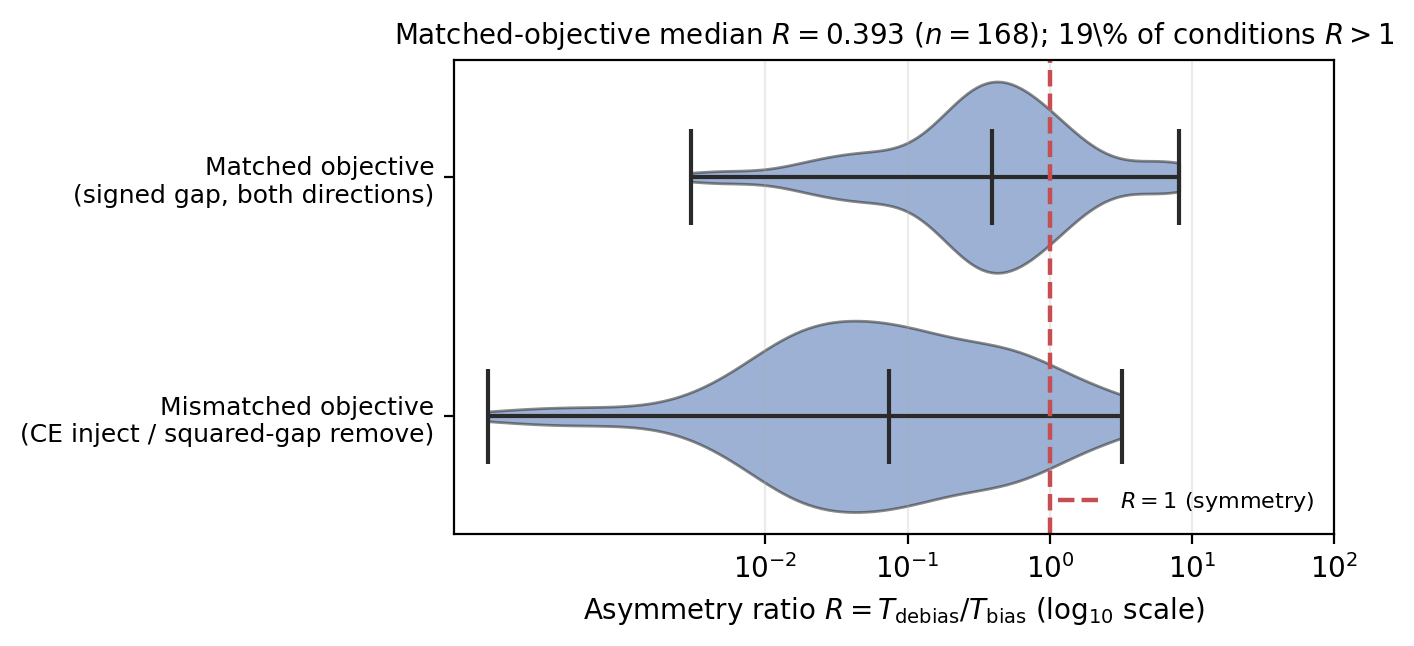
\includegraphics[width=\linewidth]{images/figure_R_distribution.png}
\caption{Distribution of the asymmetry ratio $R$ under the matched and mismatched objectives, on a $\log_{10}$ scale. The dashed line marks $R = 1$. Both distributions concentrate below one.}
\label{fig:rdist}
\end{figure}

\subsection{Censoring accounts for the reported asymmetry}

The two objectives differ sharply in one respect. Under the matched objective, injection reaches $\theta$ in every condition that starts below it, so no condition is injection-censored. Under the mismatched objective, cross-entropy injection fails to reach $\theta$ within the step budget in 49 of 180 conditions, a censoring rate of 27\%. These 49 conditions have no defined $R$. In the original protocol they did not drop out: a censored injection sets $T_{\mathrm{bias}}$ to its cap and a censored removal sets $T_{\mathrm{debias}}$ to its cap, so the pair returns a fixed ceiling ratio that the mean then averages in. A mean taken over a set that is one-quarter ceiling values sits above one even when the median of the defined values sits far below. The reported $R > 1$ is this mean, not a central tendency of measured ratios. Once censored conditions are excluded and the median is used, the asymmetry disappears.

\subsection{The pattern holds across models and languages}

Table~\ref{tab:permodel} reports $R$ by model under the matched objective. No model has a median $R$ above one. The medians range from 0.297 for mmBERT to 0.440 for XLM-RoBERTa. The share of conditions with $R > 1$ stays a minority for every model, from 3\% for IndicBERTv2 to 36\% for XLM-RoBERTa. The two models that showed the strongest apparent hysteresis under a mismatched objective, mmBERT and XLM-RoBERTa, now sit at opposite ends of this range, so the earlier ordering does not carry over to the controlled measurement.

\begin{table}[htbp]
\small\sf\centering
\caption{Matched-objective ratio $R$ by model, over converged conditions ($\theta = 0.7$). No model shows a median above one.}
\label{tab:permodel}
\begin{adjustbox}{max width=\linewidth}
\begin{tabular}{lcccc}
\toprule
\textbf{Model} & \textbf{$n$} & \textbf{Median $R$} & \textbf{$R>1$} & \textbf{Share $R>1$} \\
\midrule
mBERT & 33 & 0.392 & 9 & 0.273 \\
XLM-RoBERTa & 33 & 0.440 & 12 & 0.364 \\
MuRIL & 33 & 0.426 & 3 & 0.091 \\
IndicBERTv2 & 33 & 0.407 & 1 & 0.030 \\
mmBERT & 36 & 0.297 & 7 & 0.194 \\
\bottomrule
\end{tabular}
\end{adjustbox}
\end{table}

Table~\ref{tab:perlang} reports $R$ by language. English shows the highest median at 0.629, above Hindi at 0.333 and Bengali at 0.409, yet all three medians remain below one. The English result is closest to symmetry, consistent with the earlier observation that English biases behave differently from Hindi and Bengali, but even the English median does not cross one. The language ordering survives the control while the direction of the asymmetry does not.

\begin{table}[htbp]
\small\sf\centering
\caption{Matched-objective ratio $R$ by language, over converged conditions ($\theta = 0.7$).}
\label{tab:perlang}
\begin{adjustbox}{max width=\linewidth}
\begin{tabular}{lcccc}
\toprule
\textbf{Language} & \textbf{$n$} & \textbf{Median $R$} & \textbf{$R>1$} & \textbf{Share $R>1$} \\
\midrule
English & 54 & 0.629 & 14 & 0.259 \\
Hindi & 54 & 0.333 & 5 & 0.093 \\
Bengali & 60 & 0.409 & 13 & 0.217 \\
\bottomrule
\end{tabular}
\end{adjustbox}
\end{table}

\subsection{Gradient norms set the direction}

The reversal has a simple mechanical cause. Removal starts from the injected checkpoint, where the stereotypical and anti-stereotypical log-probabilities differ by a large margin, so the signed gap $\delta$ is large and its gradient is large. Injection starts from a near-neutral checkpoint, where the gap is small and its gradient is small. Larger gradients move the score faster. The gradient $L_2$ norm during removal exceeds that during injection by a median factor of 1.115, and a Wilcoxon signed-rank test on the paired norms confirms the difference ($p = 1\times10^{-11}$). The step count therefore encodes the gradient scale of each starting state. The ratio $R$ compares a fast reverse path against a slow forward path, and that comparison is set by where each path begins, not by any resistance in the loss landscape.

\section{Discussion}
\label{sec:discussion}

The step-count ratio $R$ has been read as evidence that bias removal is intrinsically harder than bias injection. That reading does not hold under either objective once the ratio is measured properly. The median $R$ is 0.393 under the matched objective and 0.074 under the mismatched one, and removal is the faster direction in both. The earlier $R > 1$ came from two aggregation choices rather than from the model: censored conditions were kept at their ceiling value, and the mean over a set that is one-quarter ceiling values sits above one while the median sits far below. The mismatched objective, which produced the original figures, gives the lower median here, so the effect is not a matter of matching the loss but of how the ratio is summarised.

The finding matters for how debiasing budgets are set. A pipeline that allocates extra compute to removal on the basis of a reported $R > 1$ may be responding to a measurement artefact. The safer practice is to exclude censored conditions rather than cap them, to report the median rather than the mean, and to state the objective used in each direction. The gradient-norm analysis adds a specific check: any step-count comparison between two states should account for the gradient scale at each starting point, since that scale alone can produce a ratio far from one.

\section{Conclusion}
\label{sec:conclusion}

This work tested a reported asymmetry between bias injection and bias removal on one grid under two objectives. Across 180 conditions spanning five multilingual encoders and three languages, the median $R$ is 0.393 under the matched objective and 0.074 under the mismatched one, and removal reaches the threshold faster than injection in both. The earlier $R > 1$ is an aggregation artefact: the mismatched objective leaves 27\% of conditions censored, and averaging those ceiling values pulls the mean above one while the median stays well below. A step-count ratio, summarised this way, does not measure bias hysteresis. This study is limited to encoder models with low-rank adapters and four bias categories, and full fine-tuning or generative models may behave differently. Future work will measure the loop area of a bias-field sweep, a threshold-free quantity that needs no step count, and will test whether the result holds under full fine-tuning. An asymmetry claim about bias dynamics needs censoring-aware, median-based analysis under a matched objective before it can stand.

\begin{dci}
The author declares no potential conflicts of interest with respect to the research, authorship, and publication of this article.
\end{dci}

\begin{funding}
This research received no specific grant from any funding agency in the public, commercial, or not-for-profit sectors.
\end{funding}

\bibliographystyle{SageH}
\bibliography{sample}

\end{document}
